% Title page.
\title[Aula 03]{Oceanografia Física Descritiva}
\subtitle{Dimensões dos oceanos e Propriedades físicas da água do mar}
\author[Filipe Fernandes]{Filipe P. A. Fernandes}
\institute[unimonte]{Centro Universitário Monte Serrat}
\date[Setembro 2013]{13 de Setembro 2013}

\logo{
\includegraphics[scale=0.15]{../common/university_logo.png}}

\begin{document}

% The title page frame.
\begin{frame}[plain]
  \titlepage
\end{frame}

\section*{Outline}
\begin{frame}
\tableofcontents
\end{frame}

\section{Revisão}
\begin{frame}
\frametitle{Revisão}
    \footnotesize{
    \begin{itemize}[<+-| alert@+>]
    \item[1] Introdução à Oceanografia Física
    \begin{enumerate}[<+-| alert@+>]
        \item[1.1] Objetivos da Oceanografia Física
        \item[1.2] Divisões da Oceanografia Física
        \item[1.3] Histórico da Oceanografia Física
    \end{enumerate}
    \item[2] Dimensões e formas dos oceanos
    \item[3] Propriedades físicas da água do mar
    \begin{enumerate}[<+-| alert@+>]
        \item[3.1] Temperatura
        \item[3.2] Salinidade e condutividade
        \item[3.3] Pressão
        \item[3.4] Densidade
        \item[3.5] Efeitos da temperatura, da salinidade e da pressão na
                   densidade.
    \end{enumerate}
    \end{itemize}
    }
\end{frame}

\begin{frame}
\frametitle{Revisão de termos}
\begin{itemize}
    \item {\bf Observações}: A medida direta de uma variável. Exemplo: Temperatura
          com um termômetro.
    \vspace{1.5cm}\pause
    \item {\bf Estimações}: Uma variável que é estimada a partir de outra.  Exemplo:
          Salinidade.
\end{itemize}
\end{frame}

\begin{frame}
\frametitle{Revisão de termos}
\begin{itemize}
    \item {\bf Acurácia}: A diferença entre o resultado e o valor real.
    \vspace{1.4cm}\pause
    \item {\bf Precisão}: A diferença entre um resultado e a média de várias medidas
          obtidas pelo mesmo método. Não pode ser detectado por análises
          estatísticas.
\end{itemize}
\end{frame}

\begin{frame}
\frametitle{Revisão de termos}
\begin{itemize}
    \item {\bf Erro sistemático}: Erro resultado de uma falha simples no método que
          causa os valore serem consistentemente diferentes do valor real.
    \vspace{0.7cm}\pause
    \item {\bf Error aleatório}: Resultado de limitações básicas no método. Exemplo:
          Limite da acurácias que se pode ler a marca de mercúrio num
          termômetro.  Pode ser detectado por análises estatísticas.
          Erros realmente aleatórios tem distribuição Gaussian (normal).
\end{itemize}
\end{frame}

\begin{frame}
\frametitle{Qualidade de dados (QA/QC).}
    \begin{center}
        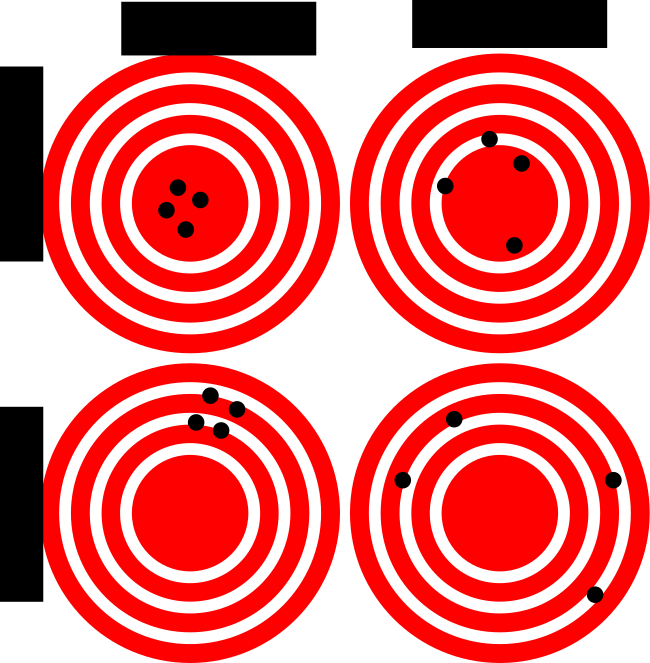
\includegraphics[scale=0.3]{./figures/accuracy_precision.pdf}
    \end{center}
    \footnotesize{Você pode corrigir a {\bf tendência mas não a imprecisão!}}
\end{frame}

\begin{frame}
\frametitle{Correção de erro sistemático.}
    \begin{center}
        \includegraphics[scale=0.35]{../figures/salinity_calibration.png}
    \end{center}
\end{frame}

\begin{frame}
\frametitle{Noções de variabilidade.}
    \begin{center}
        \includegraphics[scale=0.4]{../figures/temperature_variability.png}
    \end{center}
\end{frame}

\begin{frame}
\frametitle{Noções de variabilidade.}
    \begin{center}
        \includegraphics[scale=0.4]{../figures/salinity_variability.png}
    \end{center}
\end{frame}

\begin{frame}
\frametitle{Noções de variabilidade.}
    \begin{center}
        \includegraphics[scale=0.35]{../figures/pressure_failure.png}
    \end{center}
\end{frame}

\begin{frame}
\frametitle{Noções de variabilidade.}
    \begin{center}
        \includegraphics[scale=0.8]{../figures/wave_height.png}
    \end{center}
\end{frame}

\begin{frame}
\frametitle{Noções de variabilidade.}
    \begin{center}
        \includegraphics[scale=0.4]{../figures/current_variability_1.png}
    \end{center}
\end{frame}

\begin{frame}
\frametitle{Noções de variabilidade.}
    \begin{center}
        \includegraphics[scale=0.4]{../figures/current_variability_2.png}
    \end{center}
\end{frame}

\begin{frame}
\frametitle{Estatísticas para checar qualidade de dados.}
    \begin{center}
        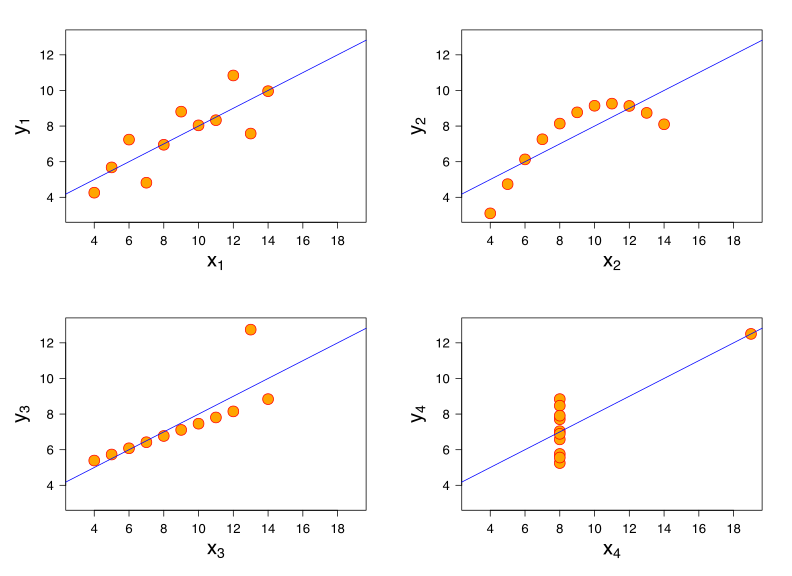
\includegraphics[scale=0.3]{./figures/anscombes_quartet_3.pdf}
%         http://en.wikipedia.org/wiki/File:Anscombe%27s_quartet_3.svg
    \end{center}
\end{frame}

\section{Coisas para lembrar!}
\begin{frame}
\frametitle{Coisas para lembrar!}
\begin{itemize}[<+-| alert@+>]
    \item Relação entre $s, t, p$ e densidade
    \item $\theta$
    \item $\sigma(s, t, p)$, $\sigma_t(s, t, 0)$ e
          $\sigma_{\theta}(s, \theta, 0)$
    \item Unidades de salinidade
    \item \bf{Pressão hidrostática}
\end{itemize}
\end{frame}

\begin{frame}
\frametitle{Coisas para lembrar!}
\begin{itemize}[<+-| alert@+>]
    \item Esquematizar perfil de temperatura
    \item Esquematizar perfil de salinidade
    \item Esquematizar perfil de densidade
    \item Explicar a equação de estado
\end{itemize}
\end{frame}

\section{Pressão hidrostática}
\begin{frame}
\frametitle{Pressão hidrostática}
    \begin{block}{Devemos interpretar as equações e não temê-las!}
    $\frac{-1}{\rho}\frac{\partial p}{\partial z} = g \rightarrow
    \int{\partial p} = g\rho \int{\partial z}
    \rightarrow p = \rho g H$
    \end{block}
    obs: Discutir como derivar usando conceitos físicos.
\end{frame}

\section{TEOS-10}
\begin{frame}
\frametitle{Salinidade Referência}
    \begin{block}{}
    É a fração de massa de material dissolvido em solução baseado
    na composição aproximada para Água do Mar Padrão.
    $\text{S}_\text{R} = (35.16504 / 35) \text{g kg}^{-1} \times \text{S}_\text{P}$
    \end{block}
\scriptsize{Millero, Frank J., et al. "The composition of Standard Seawater and the definition of the Reference-Composition Salinity Scale." Deep Sea Research Part I: Oceanographic Research Papers 55.1 (2008): 50-72.}
\end{frame}

\begin{frame}
\frametitle{Salinidade Absoluta}
    \begin{itemize}[<+-| alert@+>]
        \item A principal mudança no TEOS-10 quando comparada ao EOS-80
        \item A adoção da Salinidade Absoluta $\text{S}_\text{A}$ no lugar da
              Salinidade Prática $\text{S}_\text{P}$ (PSS-78).
    \end{itemize}
\end{frame}

\begin{frame}
\frametitle{Salinidade Absoluta}
    \begin{block}{}
        $\text{S}_\text{A} =
        \text{S}_\text{R} + \delta\text{S}_\text{A}(\phi, \lambda, p)$

        onde $\delta\text{S}_\text{A}$ é a anomalia da Salinidade em função da
        longitude, latitude e profundidade.
    \end{block}
\end{frame}

\begin{frame}
\frametitle{Salinidade Absoluta -- $\delta\text{S}_\text{A}$}
    \begin{center}
        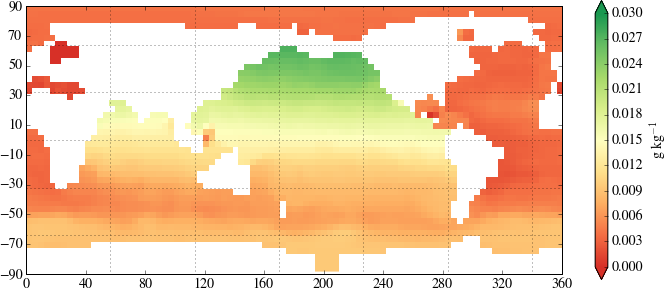
\includegraphics[scale=0.5]{./figures/delta_SA.png}
    \end{center}
\end{frame}

\begin{frame}
\frametitle{Salinidade Absoluta}
    \begin{block}{}
        Muito Importante ressaltar que apenas a Salinidade Prática (SP) deve
        ser arquivada!
    \end{block}
\end{frame}


\begin{frame}
\frametitle{Temperatura Conservativa}
    \begin{itemize}[<+-| alert@+>]
        \item As propriedades da água do mar pelo TEOS-10 é derivada da função de
              Gibbs.
        \item Por isso pode-se calcular  propriedades termodinâmicas antes
              impossível como: Entalpia, entropia, energia interna.
        \item Como entalpia é a medida de calor "verdadeiramente" conservativa.
              Oceanograficamente se criou a entalpia potencial $h^0$.
        \item Temperatura Conservativa $\Theta$ é $h^0$ dividida pela
              capacidade de calor $c_p^0$.
    \end{itemize}
\end{frame}

\begin{frame}
\frametitle{Temperatura Conservativa}
    \begin{block}{}
        Muito Importante ressaltar que apenas a temperatura {\it in situ} deve
        ser arquivada!
    \end{block}
\end{frame}

\begin{frame}
\frametitle{Temperatura Conservativa}
    \begin{center}
        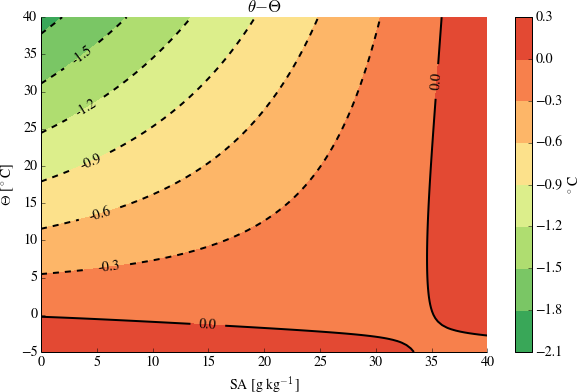
\includegraphics[scale=0.45]{./figures/conservative_temperature.png}
    \end{center}
\end{frame}

\begin{frame}
\frametitle{Dever de casa}
    \begin{block}{}
        Discussão sobre "Oscilação de Sal vs do Oscilação Campo de Vento."
    \end{block}
\end{frame}

\end{document}
